\chapter{Related Work} \label{ch:related_work}

In this chapter begins on a brief review of SDN in Section \ref{sec:sdn}.
Then we move on describing the detailed work of OpenFlow which is the first SDN standards and also the most well-known southbound protocol in Section \ref{sec:openflow}.
In Section \ref{sec:nfv}, the NFV is introduced which is a network architecture concept of relocating network functions from dedicated appliances to generic servers.

Related works of Virtual CPE platform will be described in Section \ref{sec:related_vcpe}.
We will introduce NetFATE, which our HSNL vCPE framework is inspired from. We will also introduce vCPE products proposed by Ericsson and Juniper.
Finally, we will described the HSNL vCPE framework of our laboratory, HSNL, in great detail in Section \ref{sec:hsnl_vcpe}.





\section{SDN} \label{sec:sdn}

\begin{figure}[!ht]
\centering
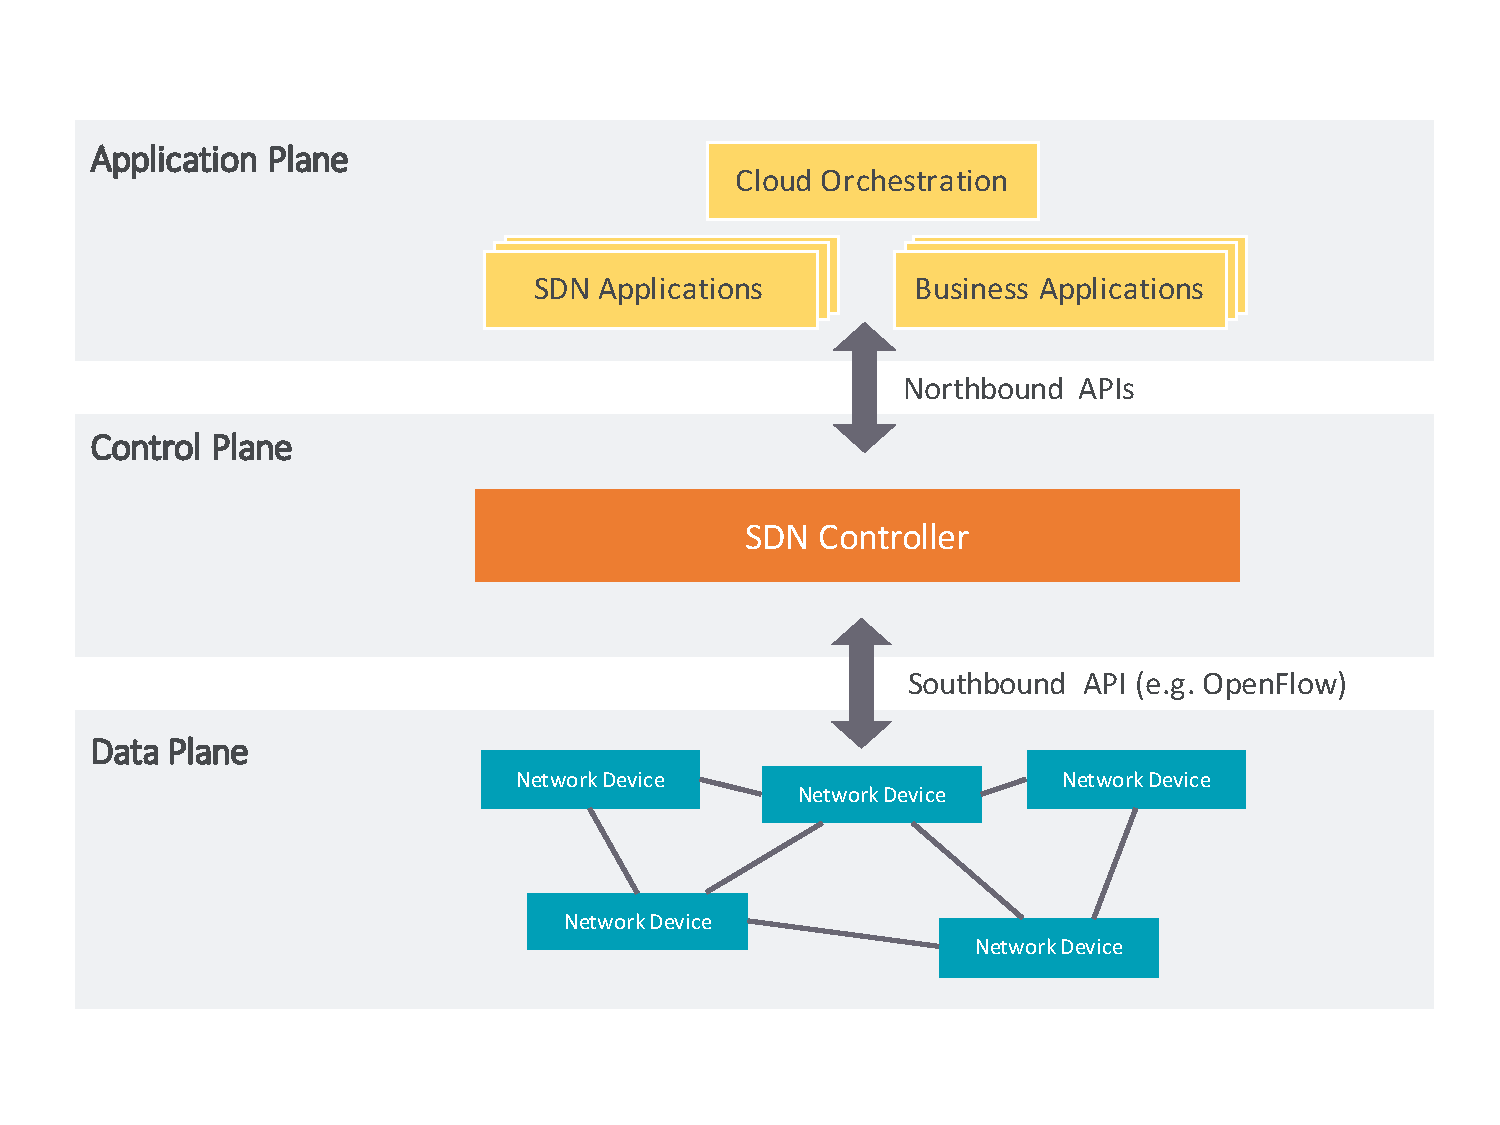
\includegraphics[width=0.9\textwidth]{./fig/sdn_architecture}
\caption{SDN logical architecture.}
\label{fig:sdn_archi}
\end{figure}

SDN has been one of the pillars of innovation in network infrastructures, allowing to decouple of the control plane and data plane and enable the programmability of the network through an open and standard interface. \cite{sdn-define}
SDN also centralizes application controls of the whole network.
With these benefits, network managers could directly implement their ideas on the network.

Figure \ref{fig:sdn_archi} depicts a logical structure view of the SDN architecture.
SDN applications and business applications are programs that built on top of the controller.
These applications performs business logic and send requests to SDN controllers through northbound APIs.
The most used northbound API is Representational State Transfer (REST) API.

When receiving the requests from applications, the SDN controller uses the southbound interface to communicate with programmable SDN network devices.
The most commonly used is the OpenFlow specification \cite{openflow-spec} defined by Open Networking Foundation (ONF) \cite{onf}, which will be presented in next section.





\section{OpenFlow Protocol} \label{sec:openflow}
\subsection{OpenFlow Switch Components}

\begin{figure}[!ht]
\centering
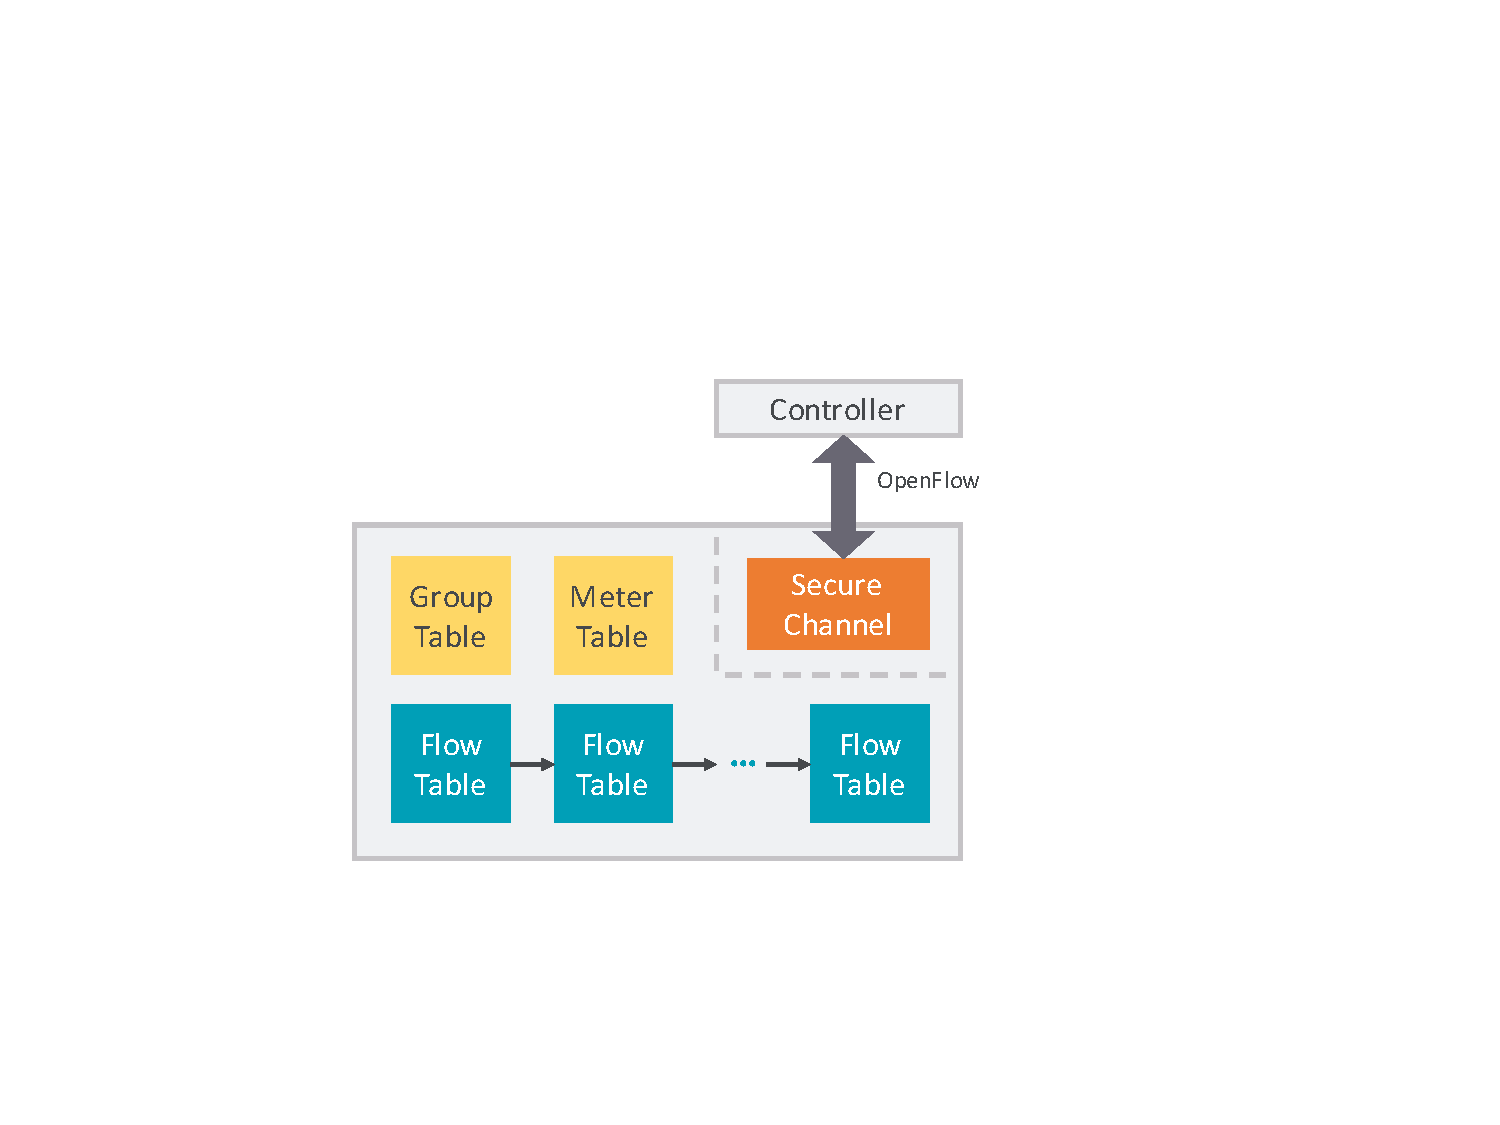
\includegraphics[width=0.5\textwidth]{./fig/openflow_switch_component}
\caption{Main components of an OpenFlow switch. \cite{openflow-spec}}
\label{fig:openflow_switch_component}
\end{figure}

Fig. \ref{fig:openflow_switch_component} illustrates basic architecture of the OpenFlow-compatible switch. In an OpenFlow Switch, there are multiple flow tables, a group table, a meter table and an OpenFlow channel.

\begin{figure}[!ht]
\centering
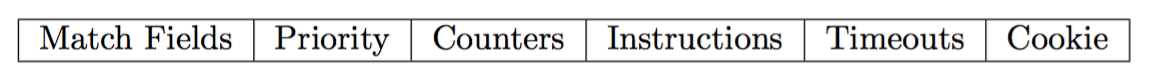
\includegraphics[width=\textwidth]{./fig/flow_entry}
\caption{Main components of a flow entry in a flow table. \cite{openflow-spec}}
\label{fig:flow_entry}
\end{figure}

There are flows entries in each flow table and each flow table entry contains match fields, priority, instructions, timeouts, and so on as shown in Fig. \ref{fig:flow_entry}.
The flow table matches incoming packets to a particular flow entry and specifies the actions that are needed to be performed on the packets.


The group table is used to arrange multiple flow entries into a group and update the actions based on the group. The meter table can trigger a variety of bandwidth performance-related actions on a flow. Through the the OpenFlow channel, SDN controller can communicates to the switch.



\subsection{Flow Table Pipeline, Matching and Table-miss}

\begin{figure}[!ht]
  % \centering
  \begin{subfigure}[b]{\textwidth}
    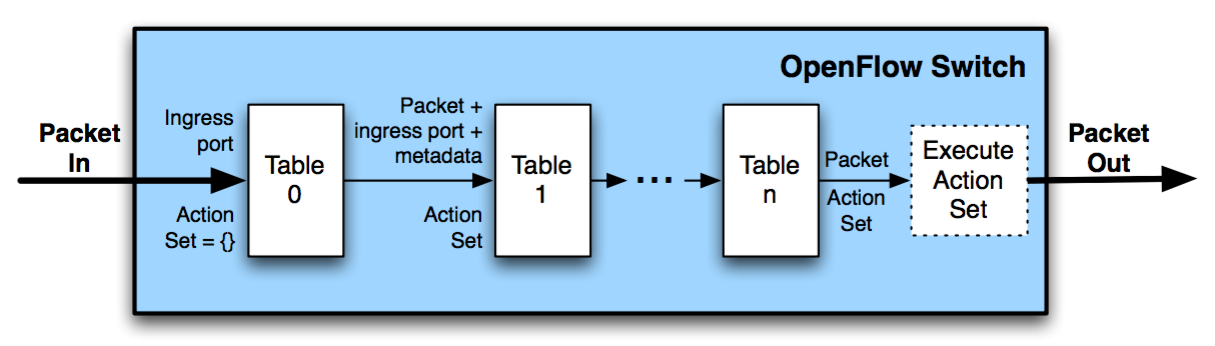
\includegraphics[width=\textwidth]{./fig/openflow_pipeline}
    \caption{Packets are matched against multiple tables in the pipeline.}
    \label{fig:openflow_pipeline2}
  \end{subfigure}
  \hfill
  \begin{subfigure}[b]{\textwidth}
    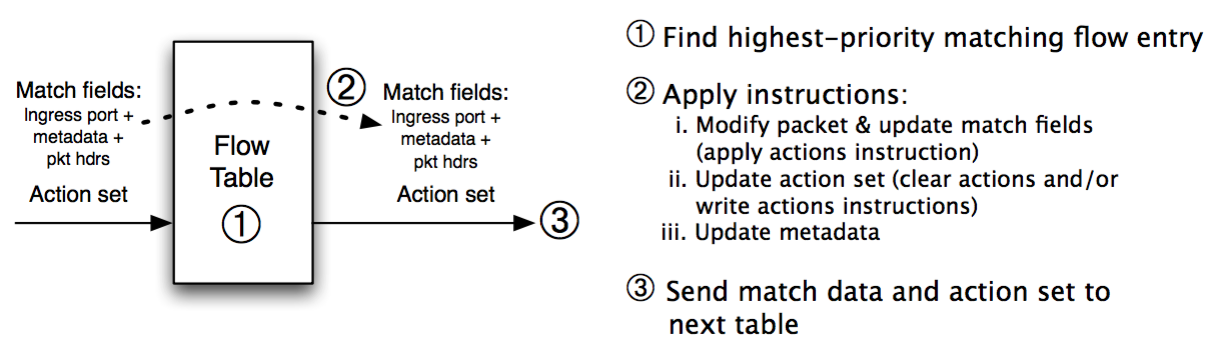
\includegraphics[width=\textwidth]{./fig/openflow_pipeline2}
    \caption{Per-table packet processing.}
    \label{fig:openflow_pipeline3}
  \end{subfigure}
  \caption{Packet flow through the processing pipeline. \cite{openflow-spec}}
  \label{fig:openflow_pipeline}
\end{figure}


\begin{figure}[!ht]
\centering
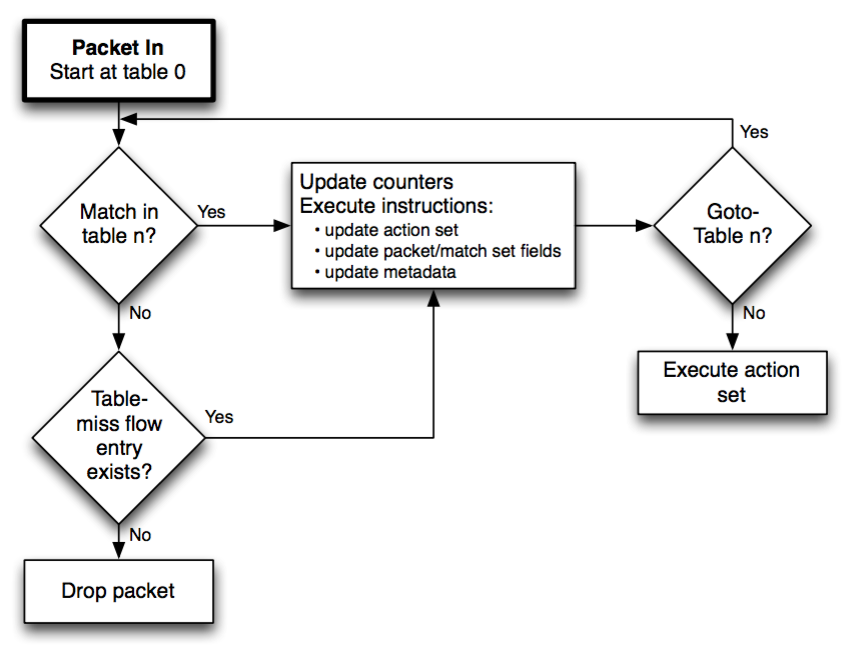
\includegraphics[width=0.9\textwidth]{./fig/openflow_matching}
\caption{The workflow of packet handling through an OpenFlow switch. \cite{openflow-spec}}
\label{fig:openflow_matching}
\end{figure}

The Packet flow through the processing pipeline is described in Fig. \ref{fig:openflow_pipeline} and the workflow of packet handling through an OpenFlow switch on receipt of a packet is illustrated in Fig. \ref{fig:openflow_matching}.

The processing of each packet always starts at the first flow table.
When being processed by a flow table, the OpenFlow switch will perform a table lookup based on the packet type, and various packet header fields, such as source MAC address or destination IP address.
If a flow table entry field has a value of ANY (field omitted), it matches all possible values in the header.
Once the packet is matched highest-priority matching flow entry in the flow table, the counters on the selected flow entry must be updated and the corresponding action must be added to the instruction set.

The packet can execute the instruction set immediately, or execute after finishing the journey in switch.
If actions applied in a previous table using the Apply-Actions changed the packet headers, those changes are applied immediately and effecting the matching in the next flow table.
A flow entry can direct a packet to next table if there's a GOTO\_TABLE action in instruction set.

Every flow table must support a table-miss flow entry to handle the table missed condition, in which packets unmatched any flow entries in the flow table. The table-miss flow entry is identified by its wildcard patterns and the lowest priority (0). The instructions of the table-miss flow entry may be sending packets to the controller (PACKET\_IN), dropping packets (DROP) or directing packets to a subsequent table (GOTO\_TABLE).




\section{NFV} \label{sec:nfv}

\begin{figure}[!ht]
\centering
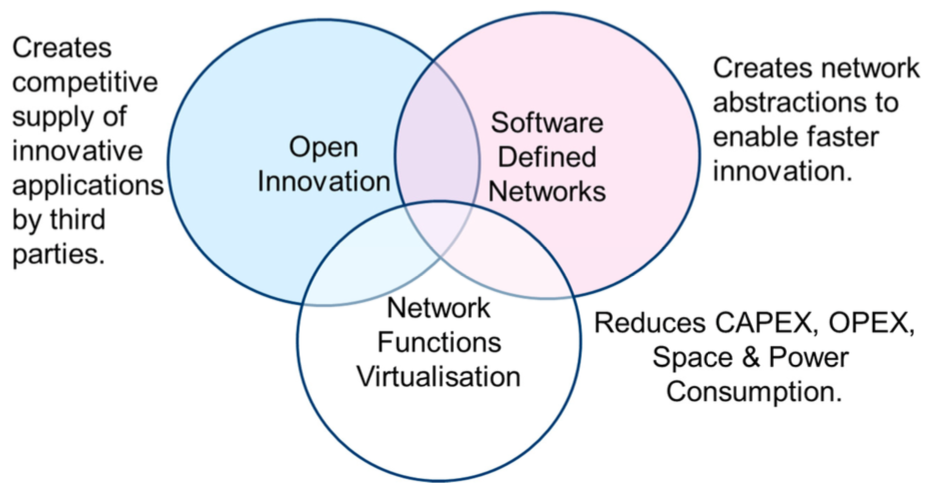
\includegraphics[width=0.9\textwidth]{./fig/nfv_and_sdn.png}
\caption{Network Functions Virtualization Relationship with SDN. \cite{nfv-wp}}
\label{fig:nfv_and_sdn}
\end{figure}

Network functions developed by different vendors and provided based on different hardware. This makes them difficult to design, manage and deploy.
To resolve these issues, telecom providers came together in a group called European Telecommunications Standards Institute (ETSI) and the ETSI setups the Industry Specification Group for Network Functions Virtualization (ISG NFV). The working group proposed a new architecture for network virtualization paradigm. The original NFV white paper \cite{nfv-wp}, described the problems that they are facing, along with their proposed solution.

NFV virtualizes network services via software and it decouples the network functions from specialized hardware and aims to replace traditional hardware-based network appliances with virtual appliances.
The benefits of network functions virtualization are: (1) reducing CapEx and OpEX, (2) encouraging more innovation and investment to bring new services quickly at much lower risk., (3) significant reduction in calls to customer support and (4) greater flexibility to scale up, scale down or evolve services





\section{Related vCPE framework} \label{sec:related_vcpe}

\subsection{ETSI NFV MANO Model}

\begin{figure}[!t]
\centering
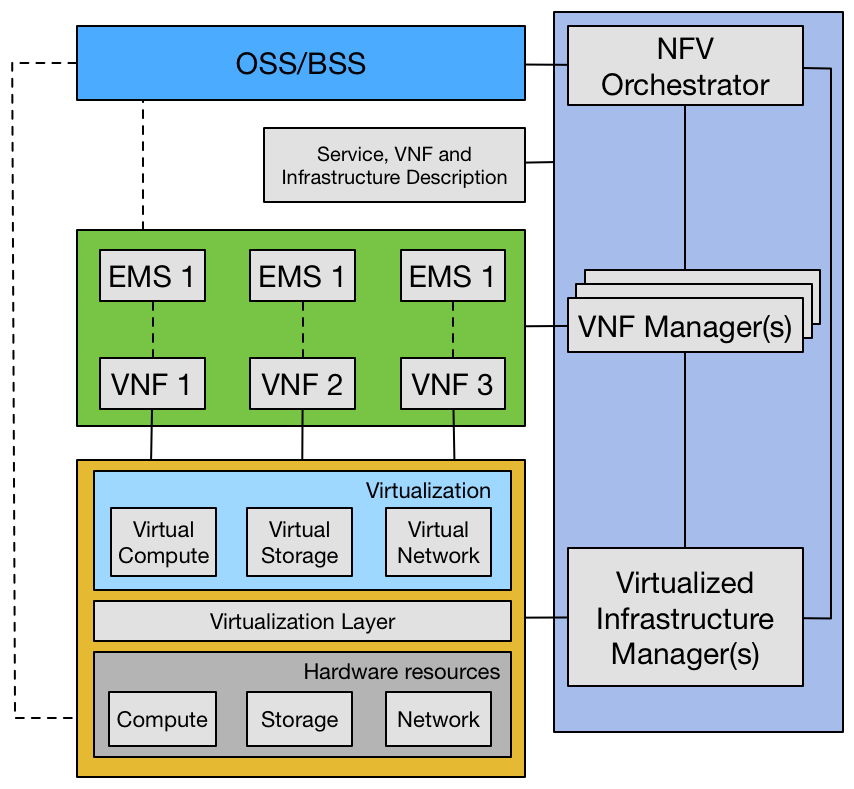
\includegraphics[width=0.9\textwidth]{./fig/etsi_nfv_architecture}
\caption{ETSI MANO Architecture. \cite{etsi-nfv-archi}}
\label{fig:etsi_nfv_architecture}
\end{figure}

Shown in Fig. \ref{fig:etsi_nfv_architecture}, the right side of the ETSI-NFV architecture \cite{etsi-nfv-archi} are: NFV Orchestrator (NFVO), VNF Manager (VNFM), and Virtualized Infrastructure Manager (VIM). NFVO is responsible for the orchestration and management of NFVI resources and to implement network services on the NFVI. VNFM is responsible for the lifecycle management of VNF instances (instantiation, configuration, update, scale up/down, termination, etc). VIM is responsible for controlling/managing the NFVI resources.

\subsection{NetFate}

NetFATE \cite{netfate}, proposed by Italy Telecom, which is a network function deploy-to-edge model in which the NFs are designed by SDN and perform by SDN switch. NetFATE architecture is compliant with the ETSI NFV architecture\cite{etsi-nfv-archi} and the so-called Virtual Network Function as a Service (VNFaaS) the NetFATE platform aims at virtualizing network functions of both CPE devices and Provider Edge (PE) nodes.

The main components of NetFATE are CPE nodes, the PE nodes, the data centers, and the orchestrator.
The CPE nodes are access gateways that can be either home gateways in a residential environment, or medium/high performance routers in an enterprise environment.
The PE nodes are the aggregation nodes of a telco network, and are typically shared by a high number of customers. Both CPE and PE nodes are included in the NFVI of NetFATE.

The orchestrator runs on a dedicated server and communicates with all the NFVI nodes through the Telco operator IP network. Its goal is to allocate, migrate and terminate VMs running network functions, and consequently controlling the traffic paths according to the run-time evolution of the network.

\begin{figure}[!ht]
\centering
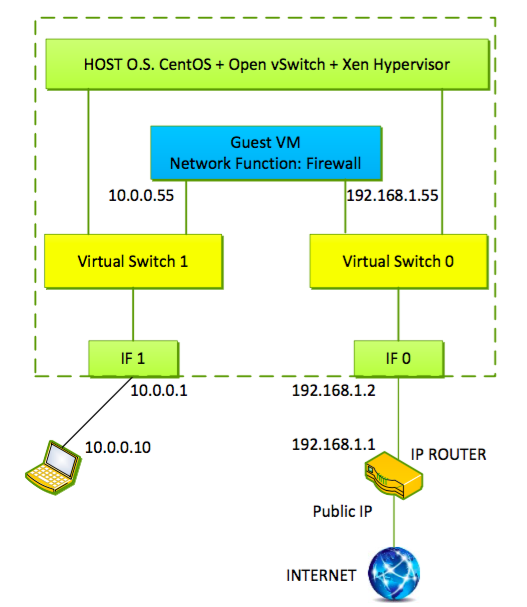
\includegraphics[width=0.8\textwidth]{./fig/netfate.png}
\caption{Virtual Firewall of NetFATE \cite{netfate}}
\label{fig:netfate}
\end{figure}

There is a case study as shown in Fig. \ref{fig:netfate} which is a virtual firewall based on the proposed NetFATE architecture. The personal virtual firewall services required by client 1 and client 2, respectively. When client 1 accesses the Internet through CPE 1 node, and then switches to the access point CPE 2 node without having any downtime. The orchestrator node in the NetFATE architecture plays a key role in the overall platform that migrates the personal virtual firewall from the previous CPE node to the new one.

The disadvantage of NetFATE is that NetFATE only tests the scenario of virtual firewall which lacks sufficient experimental results for other scenarios under NetFATE platform.




\subsection{Ericsson CPE}
Ericsson proposed a vCPE framework which achieved by unifying NFV, SDN and Cloud technologies in Internet providers’ networks and data centers \cite{ericsson-vcpe}.
On the fig. \ref{fig:ericsson_archi}, it can be seen that Ericsson vCPE solution is built from several different components: access network, cloud data center, management and orchestration, applications (Virtual Network Functions) and self-care portal.

\begin{figure}[!ht]
\centering
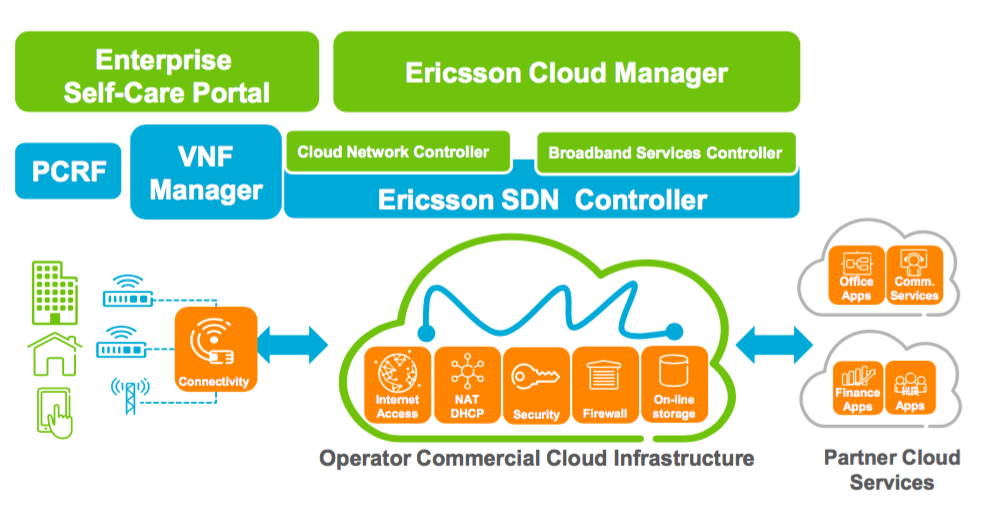
\includegraphics[width=0.9\textwidth]{./fig/ericsson_archi.png}
\caption{Ericsson vCPE architecture.\cite{ericsson-vcpe}}
\label{fig:ericsson_archi}
\end{figure}

The access network is installed on the customer location and used to identify individual end-user device.
There are 2 modes in access network: L2 tunneling mode and 2 bridge mode.
These L2 mode configurations are both used to provide CPE solution to customer.

All services functions (SFs) can be hosted as virtualized instances in an SDN enabled datacenter.
Ericsson IaaS solution is called Cloud Execution Environment (CEE), modified from OpenStack.
There are three roles in the cloud domain:
Cloud SDN switch (CSS) accepts the configuration of OpenFlow command from the SDN controllers;
Cloud SDN controller (CSC) centrally controls a network of CSS;
Broadband Service controller (BBSC) configures an SDN network through CSC and handles traffic steering along the predefined service chain.

Ericsson Cloud Manager (ECM) is used for management and orchestration, which handles business logic and subscription services.
It enables provisioning new service function instances, scaling and instantiating as requested on command.
ECM also communicate with controllers in data center to send notifications about the deployed service functions and the provisioned service chains.

Self-care portal provides the main GUI to the enterprise or home administrators for executing different service request.
Operator portal is provided towards Cloud Manager to transfer information to CEE and enterprise portal enables enterprise/home user to monitor and act on the services available.


\begin{figure}[!t]
\centering
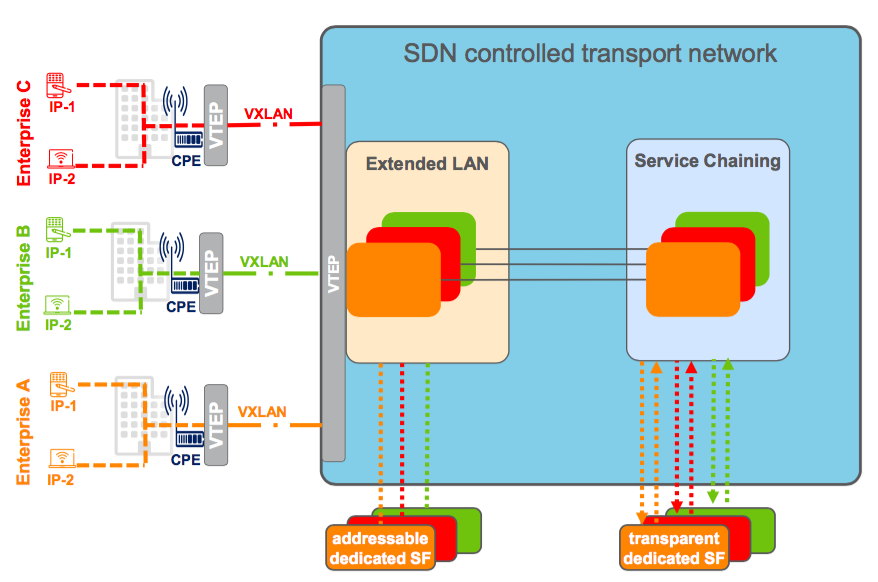
\includegraphics[width=0.9\textwidth]{./fig/ericsson_sf.png}
\caption{Overview of Service Functions.\cite{ericsson-vcpe}}
\label{fig:ericsson_sf}
\end{figure}

Then we move on to describing the SFs. There are two kinds of SFs: Addressable dedicated SF and Transparent dedicated SF, shown in Fig. \ref{fig:ericsson_sf}.
Addressable dedicated SF directly addresses end users with their MAC address.
The traffic from end-used devices will be handle by SF and forward back immediately to the end-users without the processing of service chain.
Transparent SFs use packet header to classify packet and to identify data flow.
The traffic from customers will be forward along the selected service chain.

The advantages of Ericsson vCPE solution is easy-to-deploy by using tunneling from customer to datacenter.
However, the performance of the network functions may be a concern, since all traffic is needed to forward to data center.



\subsection{Juniper Cloud CPE}
\begin{figure}[!htp]
  \centering
  \begin{subfigure}[b]{\textwidth}
    \centering
    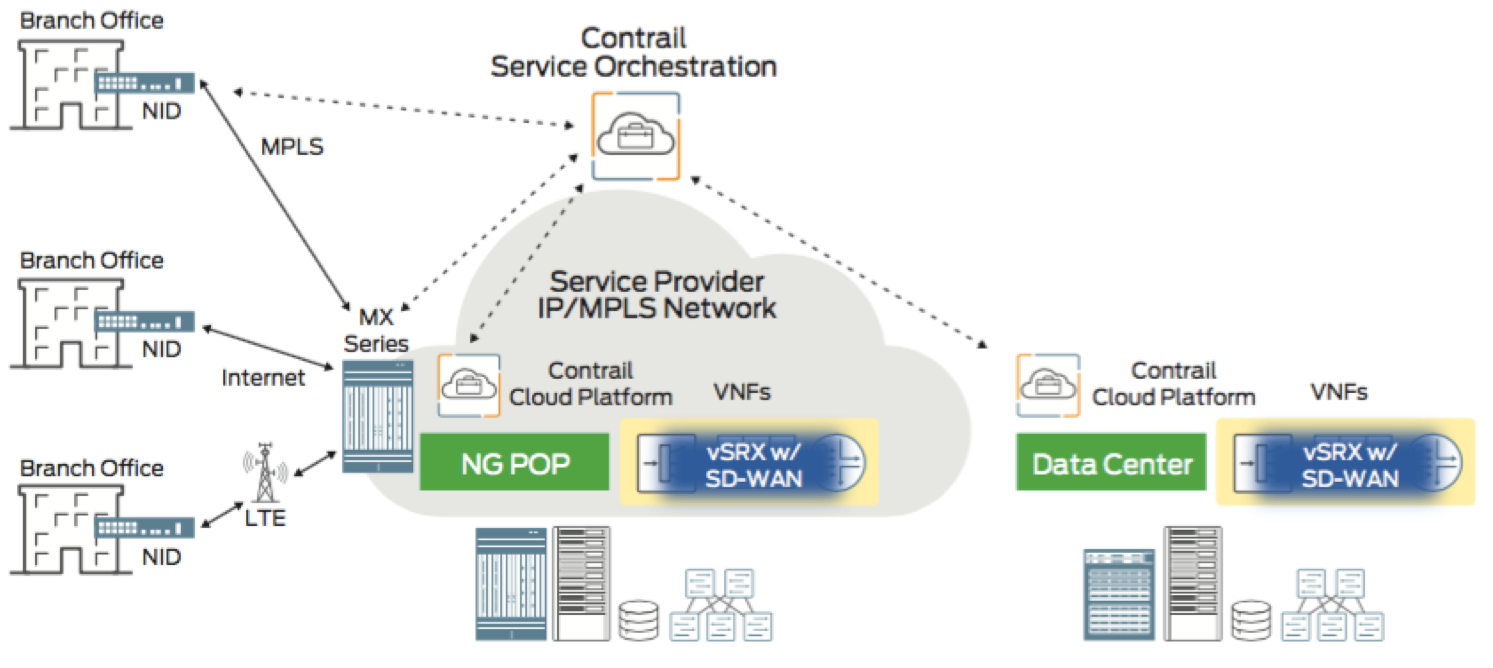
\includegraphics[width=0.9\textwidth]{./fig/juniper_central.png}
    \caption{Centralized deployment model.}
    \label{fig:juniper_central}
  \end{subfigure}
  \hfill
  \begin{subfigure}[b]{\textwidth}
    \centering
    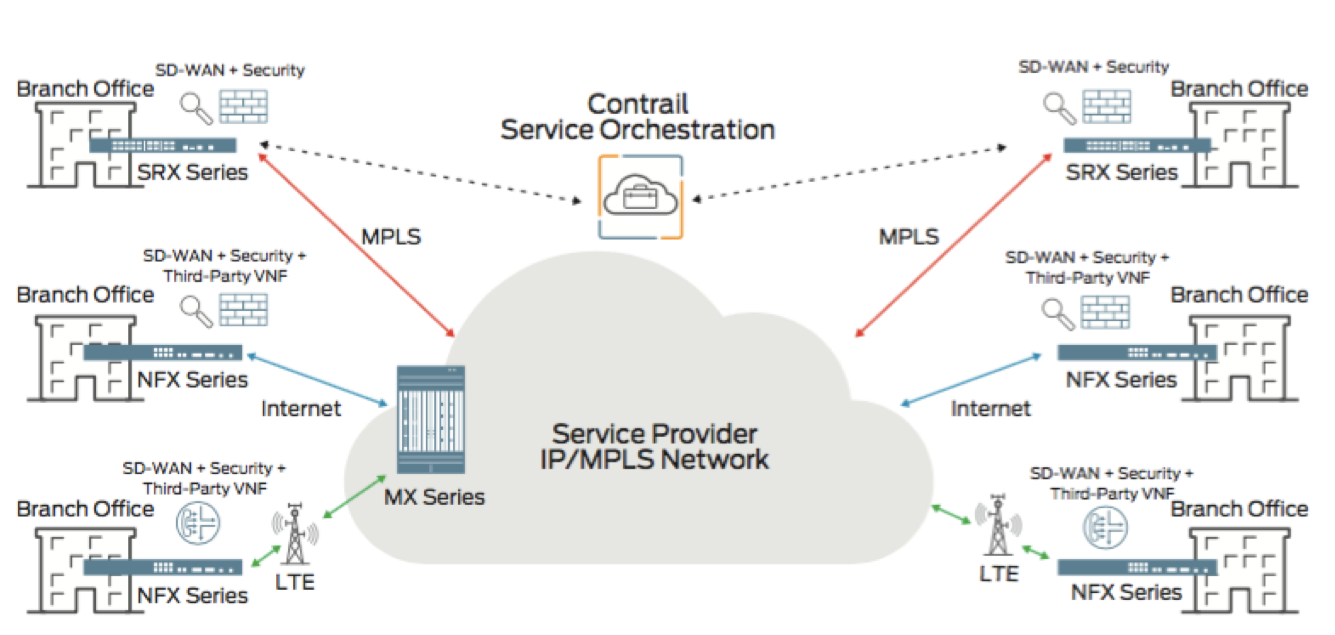
\includegraphics[width=0.9\textwidth]{./fig/juniper_distributed.png}
    \caption{Distributed deployment model.}
    \label{fig:juniper_distributed}
  \end{subfigure}
  \hfill
  \begin{subfigure}[b]{\textwidth}
    \centering
    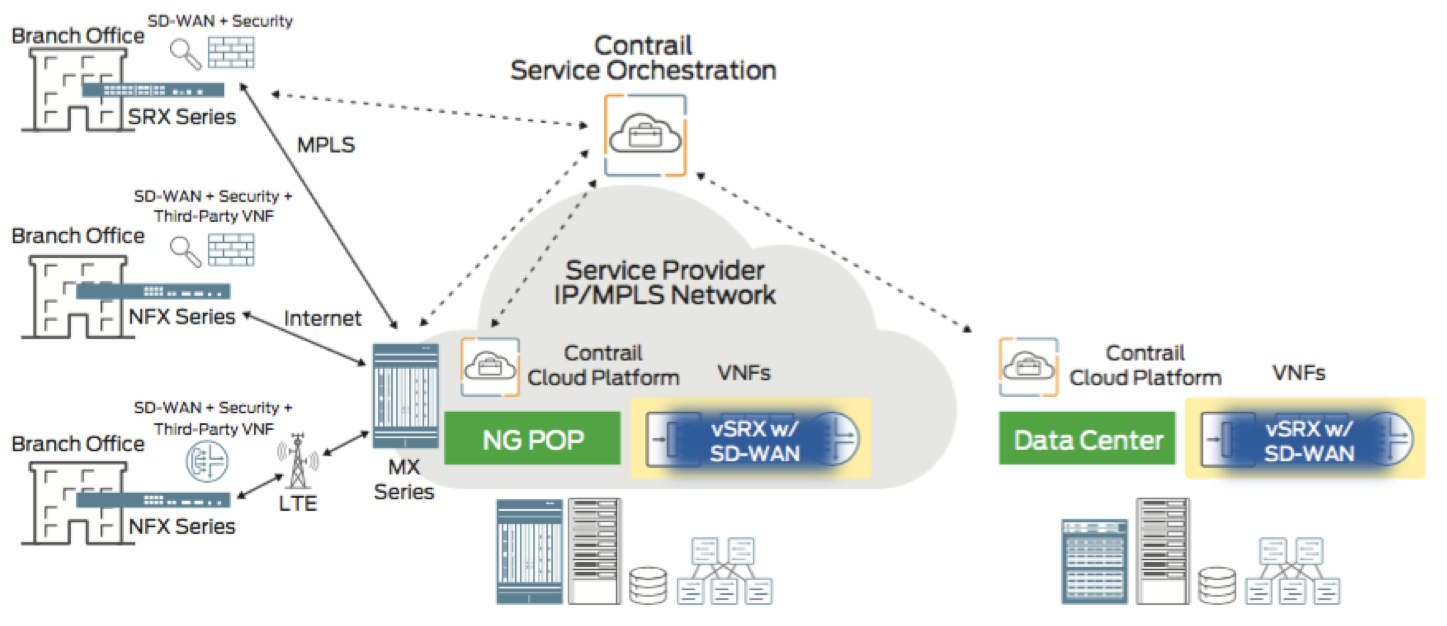
\includegraphics[width=0.9\textwidth]{./fig/juniper_hybrid.png}
    \caption{Hybrid deployment model.}
    \label{fig:juniper_hybrid}
  \end{subfigure}
  \caption{Juniper Cloud CPE deployment model. \cite{juniper-cpe}}
  \label{fig:juniper-cpe}
\end{figure}

Juniper proposed a Cloud CPE solution \cite{juniper-cpe}. There are two kinds of deployment model: centralized cloud CPE deployment model and distributed cloud CPE deployment model.

In centralized cloud CPE deployment model, services can ordered through a customer portal or trigger by existing business support system (BSS). BSS automatically instantiates VNFs and service chaining. The vCPE functions are achieved by these service chain.
In distributed cloud CPE deployment model, they distributed Juniper NFX250 service platform to customer location, which provides similar functionality to the physical CPE. A single NFX 250 device can support multiple VNFs.

Juniper’s Cloud CPE simultaneously can support both centralized and distributed model, called hybrid cloud CPE deployment model.



\section{HSNL vCPE framework} \label{sec:hsnl_vcpe}


HSNL virtual CPE platform \cite{che-wei-master, che-wei-umedia} is inspired by ETSI NFV MANO model and designed under the concept of the ETSI NFV reference architectural framework \cite{etsi-nfv-archi}.

The following part of this paper moves on to describe in greater detail the HSNL vCPE framework. Our proposed vCPE functions, which is implemented by multiple flow table management mechanism, also can be deployed by this framework.


\subsection{Deployment Model}
Unlike a related study that explored the virtualization of network function in PE devices \cite{vcpe-enhance} or used service-chains in data center to achieve vCPE services \cite{ericsson-vcpe}, HSNL introduced a network function service deployment model based on the NetFATE (Network Function at the Edge) approach \cite{netfate}.

\begin{figure}[!t]
\centering
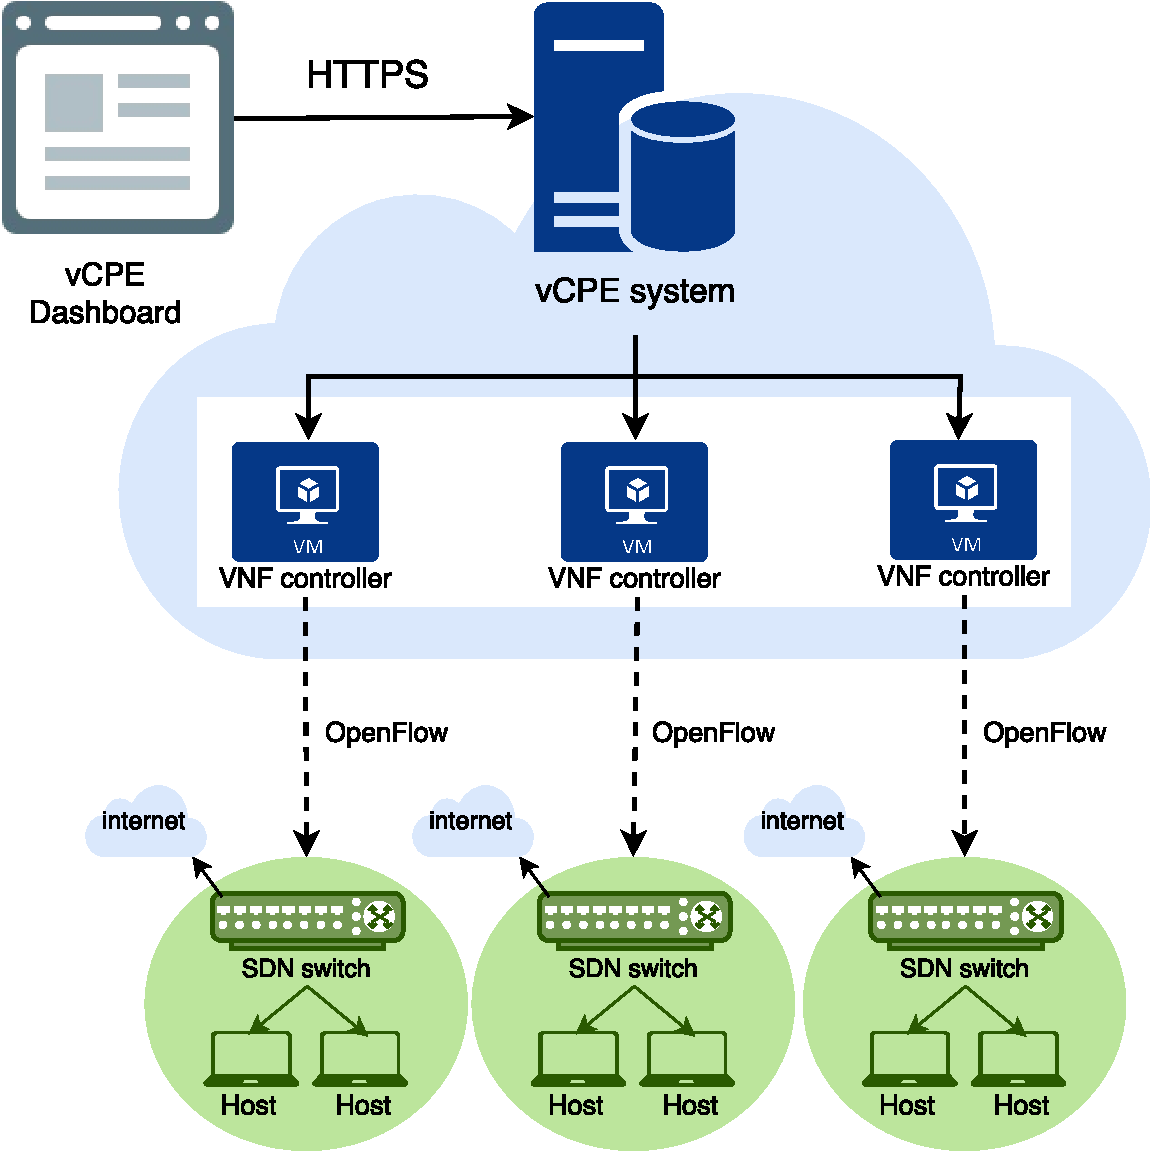
\includegraphics[width=0.9\textwidth]{./fig/hsnl_service_deployment}
\caption{Service deployment model.}
\label{fig:hsnl_service_deployment}
\end{figure}

Fig. \ref{fig:hsnl_service_deployment} illustrates the service deployment model. Each green area is a local network domain of the customer. An SDN switch is presented at the gateway of this domain. The customer can subscribe to our vCPE service through our dashboard. After subscription, the vCPE system creates a new Docker container in which an SDN controller is run. The customer only needs to set up the gateway SDN switch to connect the SDN controller through the OpenFlow protocol; thereafter, the switch executes the service.


\subsection{Architecture of the Main System}


\subsection{vCPE Platform NFV Architecture}

\begin{figure}[!t]
\centering
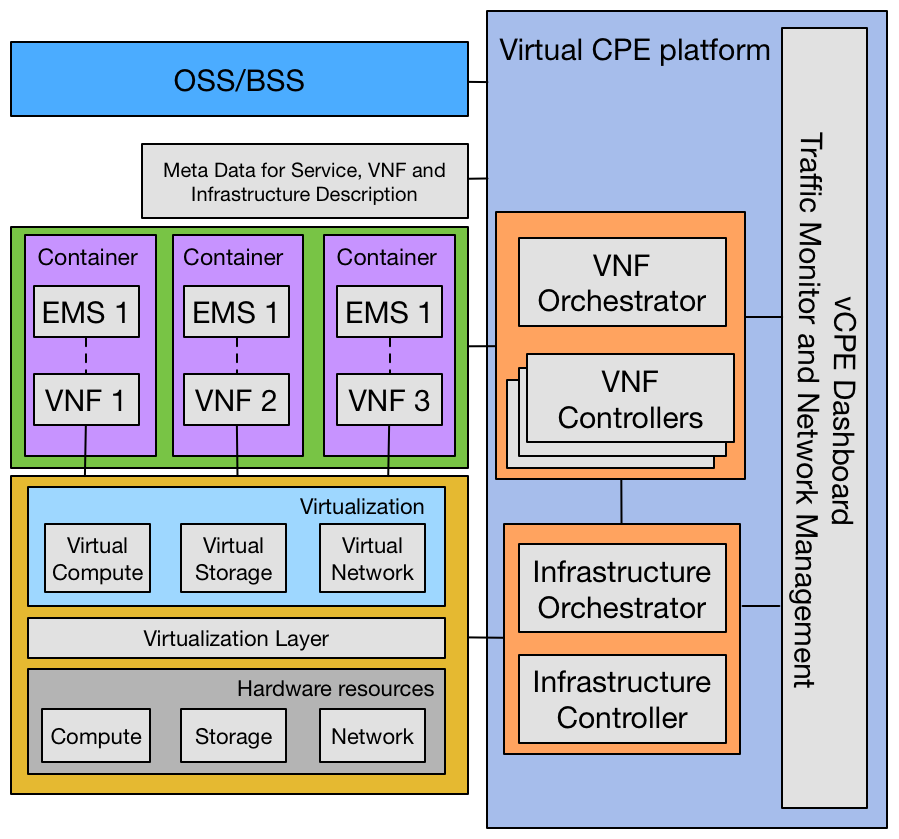
\includegraphics[width=0.9\textwidth]{./fig/hsnl_vcpe_architecture}
\caption{HSNL vCPE MANO Architecture \cite{che-wei-master}.}
\label{fig:hsnl_vcpe_architecture}
\end{figure}

The HSNL virtual CPE architecture (Fig. \ref{fig:hsnl_vcpe_architecture}) expands the scope of ETSI NFV MANO model and we will go more detail in \ref{ssec:hsnl_system_imple}.


\subsection{System Implementation} \label{ssec:hsnl_system_imple}
Turning now to the implementation of HSNL Virtual CPE platform.  The system overview (Fig. \ref{fig:hsnl_vcpe_framework}) includes an infrastructure controller, an infrastructure orchestrator, a cloud database, VNF controllers and a VNF Orchestrator. Each component is introduced in the following subsubsections.

\begin{figure}[!t]
\centering
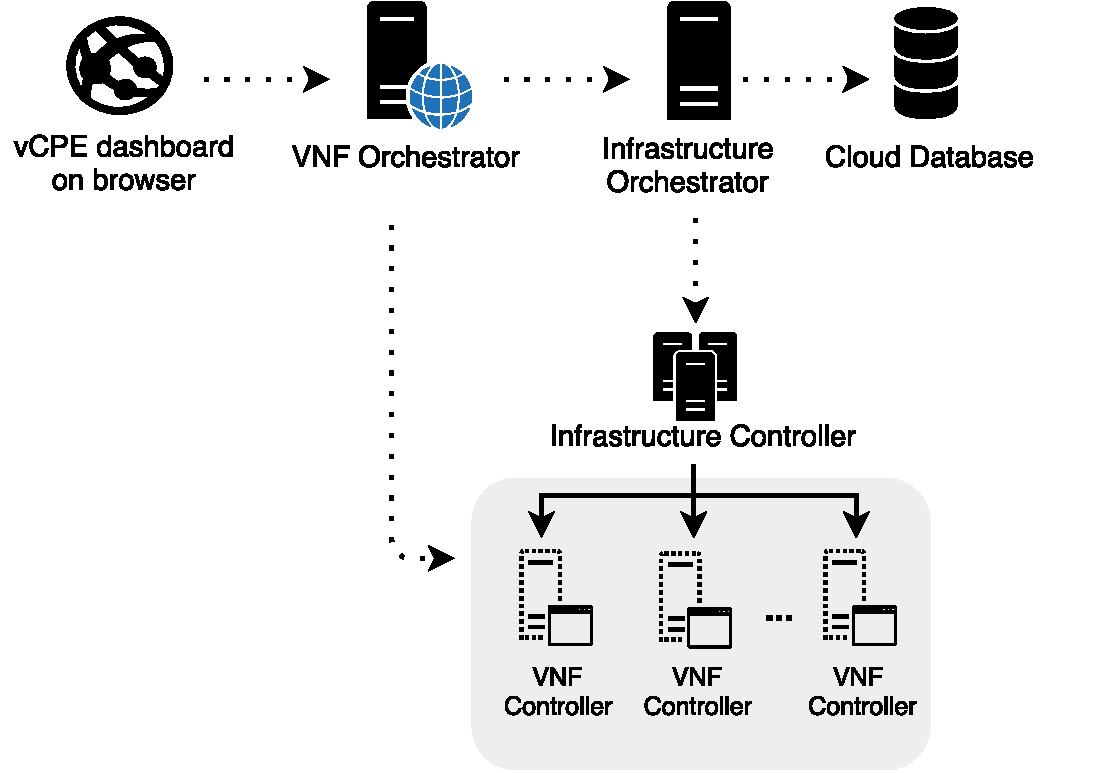
\includegraphics[width=0.9\textwidth]{./fig/hsnl_vcpe_framework}
\caption{HSNL vCPE framework overview.}
\label{fig:hsnl_vcpe_framework}
\end{figure}

\subsubsection{Infrastructure Controller}
The infrastructure controller comprises a Docker management server that can manage the Docker resources like containers and images. The infrastructure controller does not manage customer authentication or maintaining the state of the running service; it merely follows the request from the infrastructure orchestrator to create, delete, start, stop, and inspect containers.

\subsubsection{Infrastructure Orchestrator}
The infrastructure orchestrator plays a key role in our system. It connects and automates the workflows when our services are deployed. When a customer subscribes to our service, the infrastructure orchestrator first authenticates the customer, calls the infrastructure controller to create a container for the customer, and then updates the information in the database. The infrastructure orchestrator controls the entire life-cycle of our vCPE services.

\subsubsection{Cloud Database}
The cloud database is used for restoring the meta data of our vCPE services, which include each customer’s credentials, customer’s container/VM settings, and virtual CPE service states. The cloud database employs PostgreSQL, which is an open source, easily customizable and object-relational database system. Only the infrastructure orchestrator has permissions to access the cloud database.

\subsubsection{VNF Controllers}
VNF controllers comprises an SDN controller developed using Ryu framework \cite{ryu} and a remote launcher module. The original SDN controller does not have a remote launcher module for remotely executing an SDN controller. We built a light-weight server as a launcher module to resolve this problem. The remote launcher module monitors the SDN controller process ID (PID) and kills the SDN controller PID on demand. Once the infrastructure controller  creates the container, the remote module will initially runs, waiting for requests from VNF Orchestrator. The virtual CPE functions are achieved by the synergies between the VNF controller and the SDN switch.

\subsubsection{VNF Orchestrator}
The VNF orchestrator is a web application server hosted on Amazon web server, and provides to customers an online dashboard for vCPE services management and configuration. Through the web-based UI provided by the VNF orchestrator, customers can subscribe to the desired service without typing any command through the command line interface. After receiving the subscription message, the VNF orchestrator requests the infrastructure orchestrator to create a new VNF controller, and then sends the virtual CPE configuration to the new VNF controller. Based on configuration demands under different conditions, the network administrator can select any of the listed network functions on the dashboard, such as Firewall, NAT, DHCP, quality of service (QoS) management and our proposed virtual home gateway CPE functions which is implemented by multiple flow table mechanism.
